\documentclass{book}
\usepackage[a4paper,top=2.5cm,bottom=2.5cm,left=2.5cm,right=2.5cm]{geometry}
\usepackage{makeidx}
\usepackage{natbib}
\usepackage{graphicx}
\usepackage{multicol}
\usepackage{float}
\usepackage{listings}
\usepackage{color}
\usepackage{ifthen}
\usepackage[table]{xcolor}
\usepackage{textcomp}
\usepackage{alltt}
\usepackage{ifpdf}
\ifpdf
\usepackage[pdftex,
            pagebackref=true,
            colorlinks=true,
            linkcolor=blue,
            unicode
           ]{hyperref}
\else
\usepackage[ps2pdf,
            pagebackref=true,
            colorlinks=true,
            linkcolor=blue,
            unicode
           ]{hyperref}
\usepackage{pspicture}
\fi
\usepackage[utf8]{inputenc}
\usepackage{mathptmx}
\usepackage[scaled=.90]{helvet}
\usepackage{courier}
\usepackage{sectsty}
\usepackage{amssymb}
\usepackage[titles]{tocloft}
\usepackage{doxygen}
\lstset{language=C++,inputencoding=utf8,basicstyle=\footnotesize,breaklines=true,breakatwhitespace=true,tabsize=4,numbers=left }
\makeindex
\setcounter{tocdepth}{3}
\renewcommand{\footrulewidth}{0.4pt}
\renewcommand{\familydefault}{\sfdefault}
\hfuzz=15pt
\setlength{\emergencystretch}{15pt}
\hbadness=750
\tolerance=750
\begin{document}
\hypersetup{pageanchor=false,citecolor=blue}
\begin{titlepage}
\vspace*{7cm}
\begin{center}
{\Large Mercury2 Hardware Manager \\[1ex]\large 0.\-1.\-0 }\\
\vspace*{1cm}
{\large Generated by Doxygen 1.8.3}\\
\vspace*{0.5cm}
{\small Tue Jan 15 2013 15:54:12}\\
\end{center}
\end{titlepage}
\clearemptydoublepage
\pagenumbering{roman}
\tableofcontents
\clearemptydoublepage
\pagenumbering{arabic}
\hypersetup{pageanchor=true,citecolor=blue}
\chapter{Getting Started}
\label{index}\hypertarget{index}{}Mercury2 is the next generation of ground station management systems that allows users to remotely command configured ground stations over the internet. Mercury2 is composed of two primary components\-: the web based user interface, and the hardware manager.

\hyperlink{how_it_works}{How It Works} \hyperlink{installation}{Installation} 
\chapter{Configuration}
\label{Configuration}
\hypertarget{Configuration}{}
\hyperlink{core_configuration_options}{Core Configuration Options} \hyperlink{hardware_configuration}{Hardware Configuration} \hypertarget{core_configuration_options}{}\section{Core Configuration Options}\label{core_configuration_options}
\hypertarget{hardware_configuration}{}\section{Hardware Configuration}\label{hardware_configuration}

\chapter{How It Works}
\label{how_it_works}
\hypertarget{how_it_works}{}
\input{how_it_works}
\chapter{Installation}
\label{installation}
\hypertarget{installation}{}
\input{installation}
\chapter{Logging}
\label{logging}
\hypertarget{logging}{}
\hyperlink{telemetry_dumps}{Telemetry Dumps} \hypertarget{telemetry_dumps}{}\section{Telemetry Dumps}\label{telemetry_dumps}

\chapter{Security}
\label{security}
\hypertarget{security}{}
\input{security}
\chapter{Using the Ground Station}
\label{using_the_ground_station}
\hypertarget{using_the_ground_station}{}
\hyperlink{controlling_the_ground_station}{Controlling the Ground Station} \hyperlink{receiving_telemetry}{Receiving and Transmitting Telemetry} \hypertarget{controlling_the_ground_station}{}\section{Controlling the Ground Station}\label{controlling_the_ground_station}
\hyperlink{control_from_shell}{From the Shell} \hyperlink{control_from_ui}{From the User Interface} \hyperlink{command_format}{Command Format} \hypertarget{control_from_shell}{}\subsection{From the Shell}\label{control_from_shell}
\hypertarget{control_from_ui}{}\subsection{From the User Interface}\label{control_from_ui}
\hypertarget{command_format}{}\subsection{Command Format}\label{command_format}
\hypertarget{receiving_telemetry}{}\section{Receiving and Transmitting Telemetry}\label{receiving_telemetry}

\chapter{Writing Custom Drivers}
\label{writing_drivers}
\hypertarget{writing_drivers}{}
\input{writing_drivers}
\chapter{Namespace Index}
\section{Namespace List}
Here is a list of all documented namespaces with brief descriptions\-:\begin{DoxyCompactList}
\item\contentsline{section}{\hyperlink{namespacehwm_1_1command_1_1command}{hwm.\-command.\-command} \\*Contains a class used to store the state of submitted ground station commands }{\pageref{namespacehwm_1_1command_1_1command}}{}
\item\contentsline{section}{\hyperlink{namespacehwm_1_1command_1_1connection}{hwm.\-command.\-connection} \\*Contains a resource for processing commands }{\pageref{namespacehwm_1_1command_1_1connection}}{}
\item\contentsline{section}{\hyperlink{namespacehwm_1_1command_1_1handlers_1_1handler}{hwm.\-command.\-handlers.\-handler} \\*Contains the base command handler interfaces and abstract classes that all system and device command handlers should implement }{\pageref{namespacehwm_1_1command_1_1handlers_1_1handler}}{}
\item\contentsline{section}{\hyperlink{namespacehwm_1_1command_1_1handlers_1_1system}{hwm.\-command.\-handlers.\-system} \\*Contains a class that handles various system commands received by the ground station }{\pageref{namespacehwm_1_1command_1_1handlers_1_1system}}{}
\item\contentsline{section}{\hyperlink{namespacehwm_1_1command_1_1metadata}{hwm.\-command.\-metadata} \\*This module contains functions used to build a command's meta-\/data dictionary }{\pageref{namespacehwm_1_1command_1_1metadata}}{}
\item\contentsline{section}{\hyperlink{namespacehwm_1_1command_1_1parser}{hwm.\-command.\-parser} \\*Parses system and hardware commands and passes them to the appropriate command handler }{\pageref{namespacehwm_1_1command_1_1parser}}{}
\item\contentsline{section}{\hyperlink{namespacehwm_1_1core_1_1configuration}{hwm.\-core.\-configuration} \\*Contains a class to store the hardware manager configuration }{\pageref{namespacehwm_1_1core_1_1configuration}}{}
\item\contentsline{section}{\hyperlink{namespacehwm_1_1core_1_1errors}{hwm.\-core.\-errors} \\*Contains general error handling functions }{\pageref{namespacehwm_1_1core_1_1errors}}{}
\item\contentsline{section}{\hyperlink{namespacehwm_1_1core_1_1initialization}{hwm.\-core.\-initialization} \\*Initializes the Hardware Manager application }{\pageref{namespacehwm_1_1core_1_1initialization}}{}
\item\contentsline{section}{\hyperlink{namespacehwm_1_1hardware_1_1devices_1_1drivers_1_1driver}{hwm.\-hardware.\-devices.\-drivers.\-driver} \\*This module defines the base driver classes available to Mercury2 }{\pageref{namespacehwm_1_1hardware_1_1devices_1_1drivers_1_1driver}}{}
\item\contentsline{section}{\hyperlink{namespacehwm_1_1hardware_1_1devices_1_1drivers_1_1icom__910_1_1icom__910}{hwm.\-hardware.\-devices.\-drivers.\-icom\-\_\-910.\-icom\-\_\-910} \\*This module contains a hardware driver and command handler for the I\-C\-O\-M 910 radio }{\pageref{namespacehwm_1_1hardware_1_1devices_1_1drivers_1_1icom__910_1_1icom__910}}{}
\item\contentsline{section}{\hyperlink{namespacehwm_1_1hardware_1_1devices_1_1drivers_1_1kantronics__tnc_1_1kantronics__tnc}{hwm.\-hardware.\-devices.\-drivers.\-kantronics\-\_\-tnc.\-kantronics\-\_\-tnc} \\*This module contains a simple driver for Kantronics T\-N\-Cs as well as a service that it uses to report its state to other pipeline devices }{\pageref{namespacehwm_1_1hardware_1_1devices_1_1drivers_1_1kantronics__tnc_1_1kantronics__tnc}}{}
\item\contentsline{section}{\hyperlink{namespacehwm_1_1hardware_1_1devices_1_1drivers_1_1mxl__antenna__controller_1_1mxl__antenna__controller}{hwm.\-hardware.\-devices.\-drivers.\-mxl\-\_\-antenna\-\_\-controller.\-mxl\-\_\-antenna\-\_\-controller} \\*This module contains the driver and command handler for the M\-X\-L Antenna Controller }{\pageref{namespacehwm_1_1hardware_1_1devices_1_1drivers_1_1mxl__antenna__controller_1_1mxl__antenna__controller}}{}
\item\contentsline{section}{\hyperlink{namespacehwm_1_1hardware_1_1devices_1_1drivers_1_1mxl__balloon__tracker_1_1mxl__balloon__tracker}{hwm.\-hardware.\-devices.\-drivers.\-mxl\-\_\-balloon\-\_\-tracker.\-mxl\-\_\-balloon\-\_\-tracker} \\*This module contains a virtual driver that provides tracking information for M\-X\-L balloon missions using a combination of the A\-P\-R\-S.\-fi network and position information downlinked directly from the balloon }{\pageref{namespacehwm_1_1hardware_1_1devices_1_1drivers_1_1mxl__balloon__tracker_1_1mxl__balloon__tracker}}{}
\item\contentsline{section}{\hyperlink{namespacehwm_1_1hardware_1_1devices_1_1drivers_1_1service}{hwm.\-hardware.\-devices.\-drivers.\-service} \\*Provides a base abstract class that driver services may implement }{\pageref{namespacehwm_1_1hardware_1_1devices_1_1drivers_1_1service}}{}
\item\contentsline{section}{\hyperlink{namespacehwm_1_1hardware_1_1devices_1_1drivers_1_1sgp4__tracker_1_1sgp4__tracker}{hwm.\-hardware.\-devices.\-drivers.\-sgp4\-\_\-tracker.\-sgp4\-\_\-tracker} \\*This module contains a virtual driver and command handler for a standard S\-G\-P4 tracker }{\pageref{namespacehwm_1_1hardware_1_1devices_1_1drivers_1_1sgp4__tracker_1_1sgp4__tracker}}{}
\item\contentsline{section}{\hyperlink{namespacehwm_1_1hardware_1_1devices_1_1drivers_1_1test__driver_1_1test__driver}{hwm.\-hardware.\-devices.\-drivers.\-test\-\_\-driver.\-test\-\_\-driver} \\*Contains a simple empty driver for unit testing purposes }{\pageref{namespacehwm_1_1hardware_1_1devices_1_1drivers_1_1test__driver_1_1test__driver}}{}
\item\contentsline{section}{\hyperlink{namespacehwm_1_1hardware_1_1devices_1_1drivers_1_1test__virtual__driver_1_1test__virtual__driver}{hwm.\-hardware.\-devices.\-drivers.\-test\-\_\-virtual\-\_\-driver.\-test\-\_\-virtual\-\_\-driver} \\*Contains a simple empty virtual driver for unit testing purposes }{\pageref{namespacehwm_1_1hardware_1_1devices_1_1drivers_1_1test__virtual__driver_1_1test__virtual__driver}}{}
\item\contentsline{section}{\hyperlink{namespacehwm_1_1hardware_1_1devices_1_1manager}{hwm.\-hardware.\-devices.\-manager} \\*Manages access to hardware devices }{\pageref{namespacehwm_1_1hardware_1_1devices_1_1manager}}{}
\item\contentsline{section}{\hyperlink{namespacehwm_1_1hardware_1_1pipelines_1_1manager}{hwm.\-hardware.\-pipelines.\-manager} \\*Manages access to the hardware pipeline pool }{\pageref{namespacehwm_1_1hardware_1_1pipelines_1_1manager}}{}
\item\contentsline{section}{\hyperlink{namespacehwm_1_1hardware_1_1pipelines_1_1pipeline}{hwm.\-hardware.\-pipelines.\-pipeline} \\*Represents individual hardware pipelines }{\pageref{namespacehwm_1_1hardware_1_1pipelines_1_1pipeline}}{}
\item\contentsline{section}{\hyperlink{namespacehwm_1_1network_1_1protocols_1_1data}{hwm.\-network.\-protocols.\-data} \\*This module contains the Twisted Protocol and related classes used to pass pipeline data to and from the session user }{\pageref{namespacehwm_1_1network_1_1protocols_1_1data}}{}
\item\contentsline{section}{\hyperlink{namespacehwm_1_1network_1_1protocols_1_1telemetry}{hwm.\-network.\-protocols.\-telemetry} \\*This module contains the Twisted Protocol (and related classes) used to broadcast pipeline telemetry to its users }{\pageref{namespacehwm_1_1network_1_1protocols_1_1telemetry}}{}
\item\contentsline{section}{\hyperlink{namespacehwm_1_1network_1_1protocols_1_1utilities}{hwm.\-network.\-protocols.\-utilities} \\*Contains methods commonly used by the H\-W\-M network protocols }{\pageref{namespacehwm_1_1network_1_1protocols_1_1utilities}}{}
\item\contentsline{section}{\hyperlink{namespacehwm_1_1network_1_1security_1_1permissions}{hwm.\-network.\-security.\-permissions} \\*This module contains a class used to manage and cache user command permissions }{\pageref{namespacehwm_1_1network_1_1security_1_1permissions}}{}
\item\contentsline{section}{\hyperlink{namespacehwm_1_1network_1_1security_1_1verification}{hwm.\-network.\-security.\-verification} \\*Contains functions for verifying user authorization credentials }{\pageref{namespacehwm_1_1network_1_1security_1_1verification}}{}
\item\contentsline{section}{\hyperlink{namespacehwm_1_1sessions_1_1coordinator}{hwm.\-sessions.\-coordinator} \\*Coordinates various periodic tasks used by the hardware manager }{\pageref{namespacehwm_1_1sessions_1_1coordinator}}{}
\item\contentsline{section}{\hyperlink{namespacehwm_1_1sessions_1_1schedule}{hwm.\-sessions.\-schedule} \\*Stores and maintains the reservation access schedule }{\pageref{namespacehwm_1_1sessions_1_1schedule}}{}
\item\contentsline{section}{\hyperlink{namespacehwm_1_1sessions_1_1session}{hwm.\-sessions.\-session} \\*Provides a representation for hardware manager usage sessions }{\pageref{namespacehwm_1_1sessions_1_1session}}{}
\end{DoxyCompactList}

\chapter{Hierarchical Index}
\section{Class Hierarchy}
This inheritance list is sorted roughly, but not completely, alphabetically\-:\begin{DoxyCompactList}
\item \contentsline{section}{hwm.\-command.\-command.\-Command}{\pageref{classhwm_1_1command_1_1command_1_1_command}}{}
\item Command\-Handler\begin{DoxyCompactList}
\item \contentsline{section}{hwm.\-command.\-tests.\-utilities.\-Test\-Command\-Handler}{\pageref{classhwm_1_1command_1_1tests_1_1utilities_1_1_test_command_handler}}{}
\end{DoxyCompactList}
\item \contentsline{section}{hwm.\-command.\-parser.\-Command\-Parser}{\pageref{classhwm_1_1command_1_1parser_1_1_command_parser}}{}
\item \contentsline{section}{hwm.\-core.\-configuration.\-Config}{\pageref{classhwm_1_1core_1_1configuration_1_1_config}}{}
\item Device\-Command\-Handler\begin{DoxyCompactList}
\item \contentsline{section}{hwm.\-hardware.\-devices.\-drivers.\-icom\-\_\-910.\-icom\-\_\-910.\-I\-C\-O\-M910\-Handler}{\pageref{classhwm_1_1hardware_1_1devices_1_1drivers_1_1icom__910_1_1icom__910_1_1_i_c_o_m910_handler}}{}
\item \contentsline{section}{hwm.\-hardware.\-devices.\-drivers.\-mxl\-\_\-antenna\-\_\-controller.\-mxl\-\_\-antenna\-\_\-controller.\-Antenna\-Controller\-Handler}{\pageref{classhwm_1_1hardware_1_1devices_1_1drivers_1_1mxl__antenna__controller_1_1mxl__antenna__controll042461b90848f732dc4817f26065c532}}{}
\item \contentsline{section}{hwm.\-hardware.\-devices.\-drivers.\-mxl\-\_\-balloon\-\_\-tracker.\-mxl\-\_\-balloon\-\_\-tracker.\-Balloon\-Handler}{\pageref{classhwm_1_1hardware_1_1devices_1_1drivers_1_1mxl__balloon__tracker_1_1mxl__balloon__tracker_1_1_balloon_handler}}{}
\item \contentsline{section}{hwm.\-hardware.\-devices.\-drivers.\-sgp4\-\_\-tracker.\-sgp4\-\_\-tracker.\-S\-G\-P4\-Handler}{\pageref{classhwm_1_1hardware_1_1devices_1_1drivers_1_1sgp4__tracker_1_1sgp4__tracker_1_1_s_g_p4_handler}}{}
\end{DoxyCompactList}
\item \contentsline{section}{hwm.\-hardware.\-devices.\-manager.\-Device\-Manager}{\pageref{classhwm_1_1hardware_1_1devices_1_1manager_1_1_device_manager}}{}
\item Exception\begin{DoxyCompactList}
\item \contentsline{section}{hwm.\-command.\-command.\-Command\-Error}{\pageref{classhwm_1_1command_1_1command_1_1_command_error}}{}
\item \contentsline{section}{hwm.\-command.\-command.\-Command\-Invalid\-Schema}{\pageref{classhwm_1_1command_1_1command_1_1_command_invalid_schema}}{}
\item \contentsline{section}{hwm.\-command.\-command.\-Command\-Malformed}{\pageref{classhwm_1_1command_1_1command_1_1_command_malformed}}{}
\item \contentsline{section}{hwm.\-command.\-command.\-Command\-Not\-Found}{\pageref{classhwm_1_1command_1_1command_1_1_command_not_found}}{}
\item \contentsline{section}{hwm.\-command.\-metadata.\-Invalid\-Command\-Address}{\pageref{classhwm_1_1command_1_1metadata_1_1_invalid_command_address}}{}
\item \contentsline{section}{hwm.\-command.\-metadata.\-Invalid\-Command\-Metadata}{\pageref{classhwm_1_1command_1_1metadata_1_1_invalid_command_metadata}}{}
\item \contentsline{section}{hwm.\-command.\-parser.\-Command\-Failed}{\pageref{classhwm_1_1command_1_1parser_1_1_command_failed}}{}
\item \contentsline{section}{hwm.\-core.\-configuration.\-Config\-File\-Malformed}{\pageref{classhwm_1_1core_1_1configuration_1_1_config_file_malformed}}{}
\item \contentsline{section}{hwm.\-core.\-configuration.\-Config\-Invalid}{\pageref{classhwm_1_1core_1_1configuration_1_1_config_invalid}}{}
\item \contentsline{section}{hwm.\-core.\-configuration.\-Option\-Not\-Found}{\pageref{classhwm_1_1core_1_1configuration_1_1_option_not_found}}{}
\item \contentsline{section}{hwm.\-core.\-configuration.\-Option\-Protected}{\pageref{classhwm_1_1core_1_1configuration_1_1_option_protected}}{}
\item \contentsline{section}{hwm.\-hardware.\-devices.\-drivers.\-driver.\-Driver\-Error}{\pageref{classhwm_1_1hardware_1_1devices_1_1drivers_1_1driver_1_1_driver_error}}{}
\begin{DoxyCompactList}
\item \contentsline{section}{hwm.\-hardware.\-devices.\-drivers.\-driver.\-Command\-Handler\-Not\-Defined}{\pageref{classhwm_1_1hardware_1_1devices_1_1drivers_1_1driver_1_1_command_handler_not_defined}}{}
\item \contentsline{section}{hwm.\-hardware.\-devices.\-drivers.\-driver.\-Device\-In\-Use}{\pageref{classhwm_1_1hardware_1_1devices_1_1drivers_1_1driver_1_1_device_in_use}}{}
\item \contentsline{section}{hwm.\-hardware.\-devices.\-drivers.\-driver.\-Pipeline\-Already\-Registered}{\pageref{classhwm_1_1hardware_1_1devices_1_1drivers_1_1driver_1_1_pipeline_already_registered}}{}
\item \contentsline{section}{hwm.\-hardware.\-devices.\-drivers.\-driver.\-Pipeline\-Not\-Registered}{\pageref{classhwm_1_1hardware_1_1devices_1_1drivers_1_1driver_1_1_pipeline_not_registered}}{}
\item \contentsline{section}{hwm.\-hardware.\-devices.\-drivers.\-driver.\-State\-Not\-Defined}{\pageref{classhwm_1_1hardware_1_1devices_1_1drivers_1_1driver_1_1_state_not_defined}}{}
\end{DoxyCompactList}
\item \contentsline{section}{hwm.\-hardware.\-devices.\-drivers.\-icom\-\_\-910.\-icom\-\_\-910.\-I\-C\-O\-M910\-Error}{\pageref{classhwm_1_1hardware_1_1devices_1_1drivers_1_1icom__910_1_1icom__910_1_1_i_c_o_m910_error}}{}
\begin{DoxyCompactList}
\item \contentsline{section}{hwm.\-hardware.\-devices.\-drivers.\-icom\-\_\-910.\-icom\-\_\-910.\-Invalid\-Target\-Position}{\pageref{classhwm_1_1hardware_1_1devices_1_1drivers_1_1icom__910_1_1icom__910_1_1_invalid_target_position}}{}
\end{DoxyCompactList}
\item \contentsline{section}{hwm.\-hardware.\-devices.\-drivers.\-mxl\-\_\-antenna\-\_\-controller.\-mxl\-\_\-antenna\-\_\-controller.\-Antenna\-Controller\-Error}{\pageref{classhwm_1_1hardware_1_1devices_1_1drivers_1_1mxl__antenna__controller_1_1mxl__antenna__controller_1_1_antenna_controller_error}}{}
\begin{DoxyCompactList}
\item \contentsline{section}{hwm.\-hardware.\-devices.\-drivers.\-mxl\-\_\-antenna\-\_\-controller.\-mxl\-\_\-antenna\-\_\-controller.\-Invalid\-Target\-Position}{\pageref{classhwm_1_1hardware_1_1devices_1_1drivers_1_1mxl__antenna__controller_1_1mxl__antenna__controller_1_1_invalid_target_position}}{}
\end{DoxyCompactList}
\item \contentsline{section}{hwm.\-hardware.\-devices.\-drivers.\-mxl\-\_\-balloon\-\_\-tracker.\-mxl\-\_\-balloon\-\_\-tracker.\-Balloon\-Tracker\-Error}{\pageref{classhwm_1_1hardware_1_1devices_1_1drivers_1_1mxl__balloon__tracker_1_1mxl__balloon__tracker_1_1_balloon_tracker_error}}{}
\begin{DoxyCompactList}
\item \contentsline{section}{hwm.\-hardware.\-devices.\-drivers.\-mxl\-\_\-balloon\-\_\-tracker.\-mxl\-\_\-balloon\-\_\-tracker.\-A\-P\-R\-S\-A\-P\-I\-Error}{\pageref{classhwm_1_1hardware_1_1devices_1_1drivers_1_1mxl__balloon__tracker_1_1mxl__balloon__tracker_1_1_a_p_r_s_a_p_i_error}}{}
\item \contentsline{section}{hwm.\-hardware.\-devices.\-drivers.\-mxl\-\_\-balloon\-\_\-tracker.\-mxl\-\_\-balloon\-\_\-tracker.\-Position\-Not\-Available}{\pageref{classhwm_1_1hardware_1_1devices_1_1drivers_1_1mxl__balloon__tracker_1_1mxl__balloon__tracker_1_1_position_not_available}}{}
\end{DoxyCompactList}
\item \contentsline{section}{hwm.\-hardware.\-devices.\-manager.\-Device\-Config\-Invalid}{\pageref{classhwm_1_1hardware_1_1devices_1_1manager_1_1_device_config_invalid}}{}
\item \contentsline{section}{hwm.\-hardware.\-devices.\-manager.\-Device\-Not\-Found}{\pageref{classhwm_1_1hardware_1_1devices_1_1manager_1_1_device_not_found}}{}
\item \contentsline{section}{hwm.\-hardware.\-devices.\-manager.\-Devices\-Already\-Initialized}{\pageref{classhwm_1_1hardware_1_1devices_1_1manager_1_1_devices_already_initialized}}{}
\item \contentsline{section}{hwm.\-hardware.\-devices.\-manager.\-Driver\-Init\-Error}{\pageref{classhwm_1_1hardware_1_1devices_1_1manager_1_1_driver_init_error}}{}
\item \contentsline{section}{hwm.\-hardware.\-devices.\-manager.\-Driver\-Not\-Found}{\pageref{classhwm_1_1hardware_1_1devices_1_1manager_1_1_driver_not_found}}{}
\item \contentsline{section}{hwm.\-hardware.\-pipelines.\-manager.\-Pipeline\-Manager\-Error}{\pageref{classhwm_1_1hardware_1_1pipelines_1_1manager_1_1_pipeline_manager_error}}{}
\begin{DoxyCompactList}
\item \contentsline{section}{hwm.\-hardware.\-pipelines.\-manager.\-Pipeline\-Not\-Found}{\pageref{classhwm_1_1hardware_1_1pipelines_1_1manager_1_1_pipeline_not_found}}{}
\item \contentsline{section}{hwm.\-hardware.\-pipelines.\-manager.\-Pipelines\-Already\-Initialized}{\pageref{classhwm_1_1hardware_1_1pipelines_1_1manager_1_1_pipelines_already_initialized}}{}
\item \contentsline{section}{hwm.\-hardware.\-pipelines.\-manager.\-Pipeline\-Schema\-Invalid}{\pageref{classhwm_1_1hardware_1_1pipelines_1_1manager_1_1_pipeline_schema_invalid}}{}
\item \contentsline{section}{hwm.\-hardware.\-pipelines.\-manager.\-Pipelines\-Not\-Defined}{\pageref{classhwm_1_1hardware_1_1pipelines_1_1manager_1_1_pipelines_not_defined}}{}
\end{DoxyCompactList}
\item \contentsline{section}{hwm.\-hardware.\-pipelines.\-pipeline.\-Pipeline\-Error}{\pageref{classhwm_1_1hardware_1_1pipelines_1_1pipeline_1_1_pipeline_error}}{}
\begin{DoxyCompactList}
\item \contentsline{section}{hwm.\-hardware.\-pipelines.\-pipeline.\-Pipeline\-Config\-Invalid}{\pageref{classhwm_1_1hardware_1_1pipelines_1_1pipeline_1_1_pipeline_config_invalid}}{}
\item \contentsline{section}{hwm.\-hardware.\-pipelines.\-pipeline.\-Pipeline\-In\-Use}{\pageref{classhwm_1_1hardware_1_1pipelines_1_1pipeline_1_1_pipeline_in_use}}{}
\item \contentsline{section}{hwm.\-hardware.\-pipelines.\-pipeline.\-Service\-Already\-Registered}{\pageref{classhwm_1_1hardware_1_1pipelines_1_1pipeline_1_1_service_already_registered}}{}
\item \contentsline{section}{hwm.\-hardware.\-pipelines.\-pipeline.\-Service\-Invalid}{\pageref{classhwm_1_1hardware_1_1pipelines_1_1pipeline_1_1_service_invalid}}{}
\item \contentsline{section}{hwm.\-hardware.\-pipelines.\-pipeline.\-Service\-Type\-Not\-Found}{\pageref{classhwm_1_1hardware_1_1pipelines_1_1pipeline_1_1_service_type_not_found}}{}
\item \contentsline{section}{hwm.\-hardware.\-pipelines.\-pipeline.\-Session\-Already\-Registered}{\pageref{classhwm_1_1hardware_1_1pipelines_1_1pipeline_1_1_session_already_registered}}{}
\end{DoxyCompactList}
\item \contentsline{section}{hwm.\-hardware.\-pipelines.\-tests.\-test\-\_\-pipeline.\-Test\-Pipeline\-Error}{\pageref{classhwm_1_1hardware_1_1pipelines_1_1tests_1_1test__pipeline_1_1_test_pipeline_error}}{}
\item \contentsline{section}{hwm.\-network.\-security.\-permissions.\-Permissions\-Error}{\pageref{classhwm_1_1network_1_1security_1_1permissions_1_1_permissions_error}}{}
\item \contentsline{section}{hwm.\-network.\-security.\-permissions.\-Permissions\-Invalid\-Schema}{\pageref{classhwm_1_1network_1_1security_1_1permissions_1_1_permissions_invalid_schema}}{}
\item \contentsline{section}{hwm.\-network.\-security.\-permissions.\-Permissions\-User\-Not\-Found}{\pageref{classhwm_1_1network_1_1security_1_1permissions_1_1_permissions_user_not_found}}{}
\item \contentsline{section}{hwm.\-sessions.\-coordinator.\-Coordinator\-Error}{\pageref{classhwm_1_1sessions_1_1coordinator_1_1_coordinator_error}}{}
\begin{DoxyCompactList}
\item \contentsline{section}{hwm.\-sessions.\-coordinator.\-Session\-Not\-Found}{\pageref{classhwm_1_1sessions_1_1coordinator_1_1_session_not_found}}{}
\end{DoxyCompactList}
\item \contentsline{section}{hwm.\-sessions.\-schedule.\-Schedule\-Error}{\pageref{classhwm_1_1sessions_1_1schedule_1_1_schedule_error}}{}
\item \contentsline{section}{hwm.\-sessions.\-session.\-Session\-Error}{\pageref{classhwm_1_1sessions_1_1session_1_1_session_error}}{}
\begin{DoxyCompactList}
\item \contentsline{section}{hwm.\-sessions.\-session.\-Protocol\-Already\-Registered}{\pageref{classhwm_1_1sessions_1_1session_1_1_protocol_already_registered}}{}
\end{DoxyCompactList}
\item \contentsline{section}{hwm.\-sessions.\-tests.\-test\-\_\-session.\-Test\-Session\-Error}{\pageref{classhwm_1_1sessions_1_1tests_1_1test__session_1_1_test_session_error}}{}
\end{DoxyCompactList}
\item H\-T\-T\-P\-Handler\begin{DoxyCompactList}
\item \contentsline{section}{hwm.\-hardware.\-devices.\-drivers.\-mxl\-\_\-antenna\-\_\-controller.\-tests.\-test\-\_\-mxl\-\_\-antenna\-\_\-controller.\-Mock\-Antenna\-Controller\-Handler}{\pageref{classhwm_1_1hardware_1_1devices_1_1drivers_1_1mxl__antenna__controller_1_1tests_1_1test__mxl__an4ff39621ad95421d0c0b0546fd5c2e95}}{}
\item \contentsline{section}{hwm.\-hardware.\-devices.\-drivers.\-mxl\-\_\-balloon\-\_\-tracker.\-tests.\-test\-\_\-mxl\-\_\-balloon\-\_\-tracker.\-Mock\-A\-P\-R\-S\-Handler}{\pageref{classhwm_1_1hardware_1_1devices_1_1drivers_1_1mxl__balloon__tracker_1_1tests_1_1test__mxl__ballo80cf737b8e85ab33d541a92bea4dd93c}}{}
\end{DoxyCompactList}
\item object\begin{DoxyCompactList}
\item \contentsline{section}{hwm.\-command.\-handlers.\-handler.\-Command\-Handler}{\pageref{classhwm_1_1command_1_1handlers_1_1handler_1_1_command_handler}}{}
\begin{DoxyCompactList}
\item \contentsline{section}{hwm.\-command.\-handlers.\-handler.\-Device\-Command\-Handler}{\pageref{classhwm_1_1command_1_1handlers_1_1handler_1_1_device_command_handler}}{}
\item \contentsline{section}{hwm.\-command.\-handlers.\-system.\-System\-Command\-Handler}{\pageref{classhwm_1_1command_1_1handlers_1_1system_1_1_system_command_handler}}{}
\end{DoxyCompactList}
\item \contentsline{section}{hwm.\-hardware.\-devices.\-drivers.\-driver.\-Driver}{\pageref{classhwm_1_1hardware_1_1devices_1_1drivers_1_1driver_1_1_driver}}{}
\begin{DoxyCompactList}
\item \contentsline{section}{hwm.\-hardware.\-devices.\-drivers.\-driver.\-Hardware\-Driver}{\pageref{classhwm_1_1hardware_1_1devices_1_1drivers_1_1driver_1_1_hardware_driver}}{}
\begin{DoxyCompactList}
\item \contentsline{section}{hwm.\-hardware.\-devices.\-drivers.\-icom\-\_\-910.\-icom\-\_\-910.\-I\-C\-O\-M\-\_\-910}{\pageref{classhwm_1_1hardware_1_1devices_1_1drivers_1_1icom__910_1_1icom__910_1_1_i_c_o_m__910}}{}
\item \contentsline{section}{hwm.\-hardware.\-devices.\-drivers.\-kantronics\-\_\-tnc.\-kantronics\-\_\-tnc.\-Kantronics\-\_\-\-T\-N\-C}{\pageref{classhwm_1_1hardware_1_1devices_1_1drivers_1_1kantronics__tnc_1_1kantronics__tnc_1_1_kantronics___t_n_c}}{}
\item \contentsline{section}{hwm.\-hardware.\-devices.\-drivers.\-mxl\-\_\-antenna\-\_\-controller.\-mxl\-\_\-antenna\-\_\-controller.\-M\-X\-L\-\_\-\-Antenna\-\_\-\-Controller}{\pageref{classhwm_1_1hardware_1_1devices_1_1drivers_1_1mxl__antenna__controller_1_1mxl__antenna__controll300dc396624a0e0bda412a3b1ecea20c}}{}
\item \contentsline{section}{hwm.\-hardware.\-devices.\-drivers.\-test\-\_\-driver.\-test\-\_\-driver.\-Test\-\_\-\-Driver}{\pageref{classhwm_1_1hardware_1_1devices_1_1drivers_1_1test__driver_1_1test__driver_1_1_test___driver}}{}
\end{DoxyCompactList}
\item \contentsline{section}{hwm.\-hardware.\-devices.\-drivers.\-driver.\-Virtual\-Driver}{\pageref{classhwm_1_1hardware_1_1devices_1_1drivers_1_1driver_1_1_virtual_driver}}{}
\begin{DoxyCompactList}
\item \contentsline{section}{hwm.\-hardware.\-devices.\-drivers.\-mxl\-\_\-balloon\-\_\-tracker.\-mxl\-\_\-balloon\-\_\-tracker.\-M\-X\-L\-\_\-\-Balloon\-\_\-\-Tracker}{\pageref{classhwm_1_1hardware_1_1devices_1_1drivers_1_1mxl__balloon__tracker_1_1mxl__balloon__tracker_1_1_m_x_l___balloon___tracker}}{}
\item \contentsline{section}{hwm.\-hardware.\-devices.\-drivers.\-sgp4\-\_\-tracker.\-sgp4\-\_\-tracker.\-S\-G\-P4\-\_\-\-Tracker}{\pageref{classhwm_1_1hardware_1_1devices_1_1drivers_1_1sgp4__tracker_1_1sgp4__tracker_1_1_s_g_p4___tracker}}{}
\item \contentsline{section}{hwm.\-hardware.\-devices.\-drivers.\-test\-\_\-virtual\-\_\-driver.\-test\-\_\-virtual\-\_\-driver.\-Test\-\_\-\-Virtual\-\_\-\-Driver}{\pageref{classhwm_1_1hardware_1_1devices_1_1drivers_1_1test__virtual__driver_1_1test__virtual__driver_1_1_test___virtual___driver}}{}
\end{DoxyCompactList}
\end{DoxyCompactList}
\item \contentsline{section}{hwm.\-hardware.\-devices.\-drivers.\-service.\-Service}{\pageref{classhwm_1_1hardware_1_1devices_1_1drivers_1_1service_1_1_service}}{}
\begin{DoxyCompactList}
\item \contentsline{section}{hwm.\-hardware.\-devices.\-drivers.\-kantronics\-\_\-tnc.\-kantronics\-\_\-tnc.\-T\-N\-C\-State\-Service}{\pageref{classhwm_1_1hardware_1_1devices_1_1drivers_1_1kantronics__tnc_1_1kantronics__tnc_1_1_t_n_c_state_service}}{}
\item \contentsline{section}{hwm.\-hardware.\-devices.\-drivers.\-mxl\-\_\-balloon\-\_\-tracker.\-mxl\-\_\-balloon\-\_\-tracker.\-Direct\-\_\-\-Downlink\-\_\-\-A\-P\-R\-S\-\_\-\-Service}{\pageref{classhwm_1_1hardware_1_1devices_1_1drivers_1_1mxl__balloon__tracker_1_1mxl__balloon__tracker_1_1e3a9bc8b0b4bc235d39c93a5b84975bc}}{}
\item \contentsline{section}{hwm.\-hardware.\-devices.\-drivers.\-sgp4\-\_\-tracker.\-sgp4\-\_\-tracker.\-S\-G\-P4\-Propagation\-Service}{\pageref{classhwm_1_1hardware_1_1devices_1_1drivers_1_1sgp4__tracker_1_1sgp4__tracker_1_1_s_g_p4_propagation_service}}{}
\end{DoxyCompactList}
\item \contentsline{section}{hwm.\-hardware.\-pipelines.\-pipeline.\-Pipeline\-Telemetry\-Producer}{\pageref{classhwm_1_1hardware_1_1pipelines_1_1pipeline_1_1_pipeline_telemetry_producer}}{}
\item \contentsline{section}{hwm.\-sessions.\-tests.\-utilities.\-Mock\-Session\-Coordinator}{\pageref{classhwm_1_1sessions_1_1tests_1_1utilities_1_1_mock_session_coordinator}}{}
\end{DoxyCompactList}
\item \contentsline{section}{hwm.\-network.\-security.\-permissions.\-Permission\-Manager}{\pageref{classhwm_1_1network_1_1security_1_1permissions_1_1_permission_manager}}{}
\item \contentsline{section}{hwm.\-hardware.\-pipelines.\-pipeline.\-Pipeline}{\pageref{classhwm_1_1hardware_1_1pipelines_1_1pipeline_1_1_pipeline}}{}
\item \contentsline{section}{hwm.\-hardware.\-pipelines.\-manager.\-Pipeline\-Manager}{\pageref{classhwm_1_1hardware_1_1pipelines_1_1manager_1_1_pipeline_manager}}{}
\item \contentsline{section}{hwm.\-sessions.\-schedule.\-Schedule\-Manager}{\pageref{classhwm_1_1sessions_1_1schedule_1_1_schedule_manager}}{}
\item \contentsline{section}{hwm.\-sessions.\-session.\-Session}{\pageref{classhwm_1_1sessions_1_1session_1_1_session}}{}
\item \contentsline{section}{hwm.\-sessions.\-coordinator.\-Session\-Coordinator}{\pageref{classhwm_1_1sessions_1_1coordinator_1_1_session_coordinator}}{}
\item Test\-Case\begin{DoxyCompactList}
\item \contentsline{section}{hwm.\-command.\-handlers.\-tests.\-test\-\_\-system\-\_\-command\-\_\-handler.\-Test\-System\-Command\-Handler}{\pageref{classhwm_1_1command_1_1handlers_1_1tests_1_1test__system__command__handler_1_1_test_system_command_handler}}{}
\item \contentsline{section}{hwm.\-command.\-tests.\-test\-\_\-command\-\_\-infrastructure.\-Test\-Command\-Infrastructure}{\pageref{classhwm_1_1command_1_1tests_1_1test__command__infrastructure_1_1_test_command_infrastructure}}{}
\item \contentsline{section}{hwm.\-core.\-tests.\-test\-\_\-configuration.\-Test\-Configuration}{\pageref{classhwm_1_1core_1_1tests_1_1test__configuration_1_1_test_configuration}}{}
\item \contentsline{section}{hwm.\-hardware.\-devices.\-drivers.\-icom\-\_\-910.\-tests.\-test\-\_\-icom\-\_\-910.\-Test\-Icom910}{\pageref{classhwm_1_1hardware_1_1devices_1_1drivers_1_1icom__910_1_1tests_1_1test__icom__910_1_1_test_icom910}}{}
\item \contentsline{section}{hwm.\-hardware.\-devices.\-drivers.\-icom\-\_\-910.\-tests.\-test\-\_\-icom\-\_\-910.\-Test\-I\-C\-O\-M910\-Handler}{\pageref{classhwm_1_1hardware_1_1devices_1_1drivers_1_1icom__910_1_1tests_1_1test__icom__910_1_1_test_i_c_o_m910_handler}}{}
\item \contentsline{section}{hwm.\-hardware.\-devices.\-drivers.\-kantronics\-\_\-tnc.\-tests.\-test\-\_\-kantronics\-\_\-tnc.\-Test\-Kantronics\-T\-N\-C}{\pageref{classhwm_1_1hardware_1_1devices_1_1drivers_1_1kantronics__tnc_1_1tests_1_1test__kantronics__tnc_1_1_test_kantronics_t_n_c}}{}
\item \contentsline{section}{hwm.\-hardware.\-devices.\-drivers.\-kantronics\-\_\-tnc.\-tests.\-test\-\_\-kantronics\-\_\-tnc.\-Test\-Kantronics\-T\-N\-C\-Protocol}{\pageref{classhwm_1_1hardware_1_1devices_1_1drivers_1_1kantronics__tnc_1_1tests_1_1test__kantronics__tnc_fb887f0a11150054eea93748489d0600}}{}
\item \contentsline{section}{hwm.\-hardware.\-devices.\-drivers.\-kantronics\-\_\-tnc.\-tests.\-test\-\_\-kantronics\-\_\-tnc.\-Test\-Kantronics\-T\-N\-C\-State\-Service}{\pageref{classhwm_1_1hardware_1_1devices_1_1drivers_1_1kantronics__tnc_1_1tests_1_1test__kantronics__tnc_0c24dcd59df096de940a284b07dc7d74}}{}
\item \contentsline{section}{hwm.\-hardware.\-devices.\-drivers.\-mxl\-\_\-antenna\-\_\-controller.\-tests.\-test\-\_\-mxl\-\_\-antenna\-\_\-controller.\-Test\-M\-X\-L\-Antenna\-Controller\-Driver}{\pageref{classhwm_1_1hardware_1_1devices_1_1drivers_1_1mxl__antenna__controller_1_1tests_1_1test__mxl__an2edaee9f18a9d6c35832076cf9ff4beb}}{}
\item \contentsline{section}{hwm.\-hardware.\-devices.\-drivers.\-mxl\-\_\-antenna\-\_\-controller.\-tests.\-test\-\_\-mxl\-\_\-antenna\-\_\-controller.\-Test\-M\-X\-L\-Antenna\-Controller\-Handler}{\pageref{classhwm_1_1hardware_1_1devices_1_1drivers_1_1mxl__antenna__controller_1_1tests_1_1test__mxl__anf1b82778ca0869b41ace53be3d0454a2}}{}
\item \contentsline{section}{hwm.\-hardware.\-devices.\-drivers.\-mxl\-\_\-balloon\-\_\-tracker.\-tests.\-test\-\_\-mxl\-\_\-balloon\-\_\-tracker.\-Test\-A\-P\-R\-S\-Tracking\-Service}{\pageref{classhwm_1_1hardware_1_1devices_1_1drivers_1_1mxl__balloon__tracker_1_1tests_1_1test__mxl__ballo85cb9f09344d47402c35803686488a42}}{}
\item \contentsline{section}{hwm.\-hardware.\-devices.\-drivers.\-mxl\-\_\-balloon\-\_\-tracker.\-tests.\-test\-\_\-mxl\-\_\-balloon\-\_\-tracker.\-Test\-Balloon\-Handler}{\pageref{classhwm_1_1hardware_1_1devices_1_1drivers_1_1mxl__balloon__tracker_1_1tests_1_1test__mxl__ballo580f1655922408baf8d87971eb9118f3}}{}
\item \contentsline{section}{hwm.\-hardware.\-devices.\-drivers.\-mxl\-\_\-balloon\-\_\-tracker.\-tests.\-test\-\_\-mxl\-\_\-balloon\-\_\-tracker.\-Test\-M\-X\-L\-Balloon\-Tracker\-Driver}{\pageref{classhwm_1_1hardware_1_1devices_1_1drivers_1_1mxl__balloon__tracker_1_1tests_1_1test__mxl__ballodf60623d41e11143100d8361dee24ac6}}{}
\item \contentsline{section}{hwm.\-hardware.\-devices.\-drivers.\-sgp4\-\_\-tracker.\-tests.\-test\-\_\-sgp4\-\_\-tracker.\-Test\-S\-G\-P4\-Handler}{\pageref{classhwm_1_1hardware_1_1devices_1_1drivers_1_1sgp4__tracker_1_1tests_1_1test__sgp4__tracker_1_1_test_s_g_p4_handler}}{}
\item \contentsline{section}{hwm.\-hardware.\-devices.\-drivers.\-sgp4\-\_\-tracker.\-tests.\-test\-\_\-sgp4\-\_\-tracker.\-Test\-S\-G\-P4\-Tracker}{\pageref{classhwm_1_1hardware_1_1devices_1_1drivers_1_1sgp4__tracker_1_1tests_1_1test__sgp4__tracker_1_1_test_s_g_p4_tracker}}{}
\item \contentsline{section}{hwm.\-hardware.\-devices.\-drivers.\-sgp4\-\_\-tracker.\-tests.\-test\-\_\-sgp4\-\_\-tracker.\-Test\-S\-G\-P4\-Tracking\-Service}{\pageref{classhwm_1_1hardware_1_1devices_1_1drivers_1_1sgp4__tracker_1_1tests_1_1test__sgp4__tracker_1_1_test_s_g_p4_tracking_service}}{}
\item \contentsline{section}{hwm.\-hardware.\-devices.\-drivers.\-tests.\-test\-\_\-base\-\_\-driver\-\_\-class.\-Test\-Base\-Driver}{\pageref{classhwm_1_1hardware_1_1devices_1_1drivers_1_1tests_1_1test__base__driver__class_1_1_test_base_driver}}{}
\item \contentsline{section}{hwm.\-hardware.\-devices.\-tests.\-test\-\_\-device\-\_\-manager.\-Test\-Device\-Manager}{\pageref{classhwm_1_1hardware_1_1devices_1_1tests_1_1test__device__manager_1_1_test_device_manager}}{}
\item \contentsline{section}{hwm.\-hardware.\-pipelines.\-tests.\-test\-\_\-pipeline.\-Test\-Pipeline}{\pageref{classhwm_1_1hardware_1_1pipelines_1_1tests_1_1test__pipeline_1_1_test_pipeline}}{}
\item \contentsline{section}{hwm.\-hardware.\-pipelines.\-tests.\-test\-\_\-pipeline\-\_\-manager.\-Test\-Pipeline\-Manager}{\pageref{classhwm_1_1hardware_1_1pipelines_1_1tests_1_1test__pipeline__manager_1_1_test_pipeline_manager}}{}
\item \contentsline{section}{hwm.\-network.\-protocols.\-tests.\-test\-\_\-data\-\_\-protocol.\-Test\-Pipeline\-Data\-Protocol}{\pageref{classhwm_1_1network_1_1protocols_1_1tests_1_1test__data__protocol_1_1_test_pipeline_data_protocol}}{}
\item \contentsline{section}{hwm.\-network.\-protocols.\-tests.\-test\-\_\-protocol\-\_\-utilities.\-Test\-Protocol\-Utilities}{\pageref{classhwm_1_1network_1_1protocols_1_1tests_1_1test__protocol__utilities_1_1_test_protocol_utilities}}{}
\item \contentsline{section}{hwm.\-network.\-protocols.\-tests.\-test\-\_\-telemetry\-\_\-protocol.\-Test\-Pipeline\-Telemetry\-Protocol}{\pageref{classhwm_1_1network_1_1protocols_1_1tests_1_1test__telemetry__protocol_1_1_test_pipeline_telemetry_protocol}}{}
\item \contentsline{section}{hwm.\-network.\-security.\-tests.\-test\-\_\-permission\-\_\-manager.\-Test\-Permission\-Manager}{\pageref{classhwm_1_1network_1_1security_1_1tests_1_1test__permission__manager_1_1_test_permission_manager}}{}
\item \contentsline{section}{hwm.\-sessions.\-tests.\-test\-\_\-coordinator.\-Test\-Coordinator}{\pageref{classhwm_1_1sessions_1_1tests_1_1test__coordinator_1_1_test_coordinator}}{}
\item \contentsline{section}{hwm.\-sessions.\-tests.\-test\-\_\-schedule.\-Test\-Schedule}{\pageref{classhwm_1_1sessions_1_1tests_1_1test__schedule_1_1_test_schedule}}{}
\item \contentsline{section}{hwm.\-sessions.\-tests.\-test\-\_\-session.\-Test\-Session}{\pageref{classhwm_1_1sessions_1_1tests_1_1test__session_1_1_test_session}}{}
\end{DoxyCompactList}
\item Factory\begin{DoxyCompactList}
\item \contentsline{section}{hwm.\-network.\-protocols.\-data.\-Pipeline\-Data\-Factory}{\pageref{classhwm_1_1network_1_1protocols_1_1data_1_1_pipeline_data_factory}}{}
\item \contentsline{section}{hwm.\-network.\-protocols.\-telemetry.\-Pipeline\-Telemetry\-Factory}{\pageref{classhwm_1_1network_1_1protocols_1_1telemetry_1_1_pipeline_telemetry_factory}}{}
\end{DoxyCompactList}
\item Line\-Receiver\begin{DoxyCompactList}
\item \contentsline{section}{hwm.\-hardware.\-devices.\-drivers.\-kantronics\-\_\-tnc.\-kantronics\-\_\-tnc.\-Kantronics\-T\-N\-C\-Protocol}{\pageref{classhwm_1_1hardware_1_1devices_1_1drivers_1_1kantronics__tnc_1_1kantronics__tnc_1_1_kantronics_t_n_c_protocol}}{}
\end{DoxyCompactList}
\item Magic\-Mock\begin{DoxyCompactList}
\item \contentsline{section}{hwm.\-hardware.\-devices.\-drivers.\-icom\-\_\-910.\-tests.\-test\-\_\-icom\-\_\-910.\-Test\-Icom910.\-Test\-Hamlib\-Rig}{\pageref{classhwm_1_1hardware_1_1devices_1_1drivers_1_1icom__910_1_1tests_1_1test__icom__910_1_1_test_icom910_1_1_test_hamlib_rig}}{}
\end{DoxyCompactList}
\item Protocol\begin{DoxyCompactList}
\item \contentsline{section}{hwm.\-network.\-protocols.\-data.\-Pipeline\-Data}{\pageref{classhwm_1_1network_1_1protocols_1_1data_1_1_pipeline_data}}{}
\item \contentsline{section}{hwm.\-network.\-protocols.\-telemetry.\-Pipeline\-Telemetry}{\pageref{classhwm_1_1network_1_1protocols_1_1telemetry_1_1_pipeline_telemetry}}{}
\end{DoxyCompactList}
\item Resource\begin{DoxyCompactList}
\item \contentsline{section}{hwm.\-command.\-connection.\-Command\-Resource}{\pageref{classhwm_1_1command_1_1connection_1_1_command_resource}}{}
\end{DoxyCompactList}
\end{DoxyCompactList}

\chapter{Class Index}
\section{Class List}
Here are the classes, structs, unions and interfaces with brief descriptions\-:\begin{DoxyCompactList}
\item\contentsline{section}{\hyperlink{classhwm_1_1network_1_1command_1_1factory_1_1_command_factory}{hwm.\-network.\-command.\-factory.\-Command\-Factory} \\*Manages command protocol instances as needed }{\pageref{classhwm_1_1network_1_1command_1_1factory_1_1_command_factory}}{}
\item\contentsline{section}{\hyperlink{classhwm_1_1core_1_1configuration_1_1_config}{hwm.\-core.\-configuration.\-Config} \\*Provides access to the hardware manager application configuration }{\pageref{classhwm_1_1core_1_1configuration_1_1_config}}{}
\item\contentsline{section}{\hyperlink{classhwm_1_1core_1_1configuration_1_1_option_not_found}{hwm.\-core.\-configuration.\-Option\-Not\-Found} }{\pageref{classhwm_1_1core_1_1configuration_1_1_option_not_found}}{}
\item\contentsline{section}{\hyperlink{classhwm_1_1core_1_1configuration_1_1_option_protected}{hwm.\-core.\-configuration.\-Option\-Protected} }{\pageref{classhwm_1_1core_1_1configuration_1_1_option_protected}}{}
\item\contentsline{section}{\hyperlink{classhwm_1_1hardware_1_1pipelines_1_1pipeline_1_1_pipeline}{hwm.\-hardware.\-pipelines.\-pipeline.\-Pipeline} \\*Represents and provides access to hardware pipelines }{\pageref{classhwm_1_1hardware_1_1pipelines_1_1pipeline_1_1_pipeline}}{}
\item\contentsline{section}{\hyperlink{classhwm_1_1hardware_1_1pipelines_1_1pipeline_1_1_pipeline_in_use}{hwm.\-hardware.\-pipelines.\-pipeline.\-Pipeline\-In\-Use} }{\pageref{classhwm_1_1hardware_1_1pipelines_1_1pipeline_1_1_pipeline_in_use}}{}
\item\contentsline{section}{\hyperlink{classhwm_1_1hardware_1_1pipelines_1_1pipeline_1_1_pipeline_invalid_configuration}{hwm.\-hardware.\-pipelines.\-pipeline.\-Pipeline\-Invalid\-Configuration} }{\pageref{classhwm_1_1hardware_1_1pipelines_1_1pipeline_1_1_pipeline_invalid_configuration}}{}
\item\contentsline{section}{\hyperlink{classhwm_1_1hardware_1_1pipelines_1_1manager_1_1_pipeline_manager}{hwm.\-hardware.\-pipelines.\-manager.\-Pipeline\-Manager} \\*Provides access the collection of available hardware pipelines }{\pageref{classhwm_1_1hardware_1_1pipelines_1_1manager_1_1_pipeline_manager}}{}
\item\contentsline{section}{\hyperlink{classhwm_1_1hardware_1_1pipelines_1_1manager_1_1_pipeline_not_found}{hwm.\-hardware.\-pipelines.\-manager.\-Pipeline\-Not\-Found} }{\pageref{classhwm_1_1hardware_1_1pipelines_1_1manager_1_1_pipeline_not_found}}{}
\item\contentsline{section}{\hyperlink{classhwm_1_1hardware_1_1pipelines_1_1manager_1_1_pipelines_all_ready_initialized}{hwm.\-hardware.\-pipelines.\-manager.\-Pipelines\-All\-Ready\-Initialized} }{\pageref{classhwm_1_1hardware_1_1pipelines_1_1manager_1_1_pipelines_all_ready_initialized}}{}
\item\contentsline{section}{\hyperlink{classhwm_1_1hardware_1_1pipelines_1_1manager_1_1_pipelines_not_defined}{hwm.\-hardware.\-pipelines.\-manager.\-Pipelines\-Not\-Defined} }{\pageref{classhwm_1_1hardware_1_1pipelines_1_1manager_1_1_pipelines_not_defined}}{}
\item\contentsline{section}{\hyperlink{classhwm_1_1sessions_1_1schedule_1_1_schedule_error}{hwm.\-sessions.\-schedule.\-Schedule\-Error} \\*Thrown if an error occurs while updating the schedule }{\pageref{classhwm_1_1sessions_1_1schedule_1_1_schedule_error}}{}
\item\contentsline{section}{\hyperlink{classhwm_1_1sessions_1_1schedule_1_1_schedule_manager}{hwm.\-sessions.\-schedule.\-Schedule\-Manager} \\*Represents a reservation access schedule }{\pageref{classhwm_1_1sessions_1_1schedule_1_1_schedule_manager}}{}
\item\contentsline{section}{\hyperlink{classhwm_1_1sessions_1_1session_1_1_session}{hwm.\-sessions.\-session.\-Session} \\*Represents a user hardware manager usage session }{\pageref{classhwm_1_1sessions_1_1session_1_1_session}}{}
\item\contentsline{section}{\hyperlink{classhwm_1_1sessions_1_1coordinator_1_1_session_coordinator}{hwm.\-sessions.\-coordinator.\-Session\-Coordinator} \\*Handles the creation and management of reservation sessions }{\pageref{classhwm_1_1sessions_1_1coordinator_1_1_session_coordinator}}{}
\item\contentsline{section}{\hyperlink{classhwm_1_1core_1_1tests_1_1test__configuration_1_1_test_configuration}{hwm.\-core.\-tests.\-test\-\_\-configuration.\-Test\-Configuration} \\*This test case tests the functionality of the configuration module (and Config class) }{\pageref{classhwm_1_1core_1_1tests_1_1test__configuration_1_1_test_configuration}}{}
\item\contentsline{section}{\hyperlink{classhwm_1_1sessions_1_1tests_1_1test__coordinator_1_1_test_coordinator}{hwm.\-sessions.\-tests.\-test\-\_\-coordinator.\-Test\-Coordinator} \\*This test suite tests the functionality of the session coordinator }{\pageref{classhwm_1_1sessions_1_1tests_1_1test__coordinator_1_1_test_coordinator}}{}
\item\contentsline{section}{\hyperlink{classhwm_1_1hardware_1_1pipelines_1_1tests_1_1test__pipeline__manager_1_1_test_pipeline_manager}{hwm.\-hardware.\-pipelines.\-tests.\-test\-\_\-pipeline\-\_\-manager.\-Test\-Pipeline\-Manager} \\*This collection of tests tests the hardware pipeline manager, which is responsible for managing access to the individual hardware pipelines }{\pageref{classhwm_1_1hardware_1_1pipelines_1_1tests_1_1test__pipeline__manager_1_1_test_pipeline_manager}}{}
\item\contentsline{section}{\hyperlink{classhwm_1_1sessions_1_1tests_1_1test__schedule_1_1_test_schedule}{hwm.\-sessions.\-tests.\-test\-\_\-schedule.\-Test\-Schedule} \\*This test suite tests the functionality of the schedule manager (Schedule\-Manager) }{\pageref{classhwm_1_1sessions_1_1tests_1_1test__schedule_1_1_test_schedule}}{}
\end{DoxyCompactList}

\chapter{Namespace Documentation}
\hypertarget{namespacehwm_1_1application_1_1core_1_1configuration}{\section{hwm.\-application.\-core.\-configuration Namespace Reference}
\label{namespacehwm_1_1application_1_1core_1_1configuration}\index{hwm.\-application.\-core.\-configuration@{hwm.\-application.\-core.\-configuration}}
}


Contains a class to store the hardware manager configuration.  


\subsection*{Classes}
\begin{DoxyCompactItemize}
\item 
class \hyperlink{classhwm_1_1application_1_1core_1_1configuration_1_1_config}{Config}
\begin{DoxyCompactList}\small\item\em Provides access to the hardware manager application configuration. \end{DoxyCompactList}\item 
class \hyperlink{classhwm_1_1application_1_1core_1_1configuration_1_1_option_protected}{Option\-Protected}
\item 
class \hyperlink{classhwm_1_1application_1_1core_1_1configuration_1_1_option_not_found}{Option\-Not\-Found}
\end{DoxyCompactItemize}
\subsection*{Variables}
\begin{DoxyCompactItemize}
\item 
tuple \hyperlink{namespacehwm_1_1application_1_1core_1_1configuration_adda0a880b39910458ecbd29d662d1b19}{Configuration} \hyperlink{classhwm_1_1application_1_1core_1_1configuration_1_1_config}{Config}()
\begin{DoxyCompactList}\small\item\em Stores a 'singleton' instance of the \hyperlink{classhwm_1_1application_1_1core_1_1configuration_1_1_config}{Config} object. \end{DoxyCompactList}\end{DoxyCompactItemize}


\subsection{Detailed Description}
Contains a class to store the hardware manager configuration. This module contains a class that provides methods for storing, modifying, and retrieving application configuration and shared state for the hardware manager. Access it by importing the Configuration variable. 

\subsection{Variable Documentation}
\hypertarget{namespacehwm_1_1application_1_1core_1_1configuration_adda0a880b39910458ecbd29d662d1b19}{\index{hwm\-::application\-::core\-::configuration@{hwm\-::application\-::core\-::configuration}!Configuration@{Configuration}}
\index{Configuration@{Configuration}!hwm::application::core::configuration@{hwm\-::application\-::core\-::configuration}}
\subsubsection[{Configuration}]{\setlength{\rightskip}{0pt plus 5cm}tuple hwm.\-application.\-core.\-configuration.\-Configuration {\bf Config}()}}\label{namespacehwm_1_1application_1_1core_1_1configuration_adda0a880b39910458ecbd29d662d1b19}


Stores a 'singleton' instance of the \hyperlink{classhwm_1_1application_1_1core_1_1configuration_1_1_config}{Config} object. 

Assign local references to this instance to access the configuration. 
\hypertarget{namespacehwm_1_1application_1_1core_1_1errors}{\section{hwm.\-application.\-core.\-errors Namespace Reference}
\label{namespacehwm_1_1application_1_1core_1_1errors}\index{hwm.\-application.\-core.\-errors@{hwm.\-application.\-core.\-errors}}
}


Contains general error handling functions.  


\subsection*{Functions}
\begin{DoxyCompactItemize}
\item 
def \hyperlink{namespacehwm_1_1application_1_1core_1_1errors_a10d031e79f3534b5a7c704a658eec281}{uncaught\-\_\-exception}
\begin{DoxyCompactList}\small\item\em Handles previously uncaught exceptions. \end{DoxyCompactList}\end{DoxyCompactItemize}


\subsection{Detailed Description}
Contains general error handling functions. This module contains assorted error handling functions. These functions are typically used to handle top-\/level hardware manager exceptions (such as a previously uncaught exceptions). 

\subsection{Function Documentation}
\hypertarget{namespacehwm_1_1application_1_1core_1_1errors_a10d031e79f3534b5a7c704a658eec281}{\index{hwm\-::application\-::core\-::errors@{hwm\-::application\-::core\-::errors}!uncaught\-\_\-exception@{uncaught\-\_\-exception}}
\index{uncaught\-\_\-exception@{uncaught\-\_\-exception}!hwm::application::core::errors@{hwm\-::application\-::core\-::errors}}
\subsubsection[{uncaught\-\_\-exception}]{\setlength{\rightskip}{0pt plus 5cm}def hwm.\-application.\-core.\-errors.\-uncaught\-\_\-exception (
\begin{DoxyParamCaption}
\item[{}]{type, }
\item[{}]{value, }
\item[{}]{tb}
\end{DoxyParamCaption}
)}}\label{namespacehwm_1_1application_1_1core_1_1errors_a10d031e79f3534b5a7c704a658eec281}


Handles previously uncaught exceptions. 

This method is used to handle top-\/level uncaught exceptions. It exits the program with an error code if such an exception is encountered.

\begin{DoxyNote}{Note}
This function logs all uncaught exceptions to the application logs, which are set up in \hyperlink{namespacehwm_1_1application_1_1core_1_1initialization}{hwm.\-application.\-core.\-initialization}. If the logs haven't been set up (i.\-e. the exception was generated early on) the default log settings will be used.
\end{DoxyNote}

\begin{DoxyParams}{Parameters}
{\em type} & The exception type. \\
\hline
{\em value} & The exception descriptive text. \\
\hline
{\em tb} & The complete traceback for the provided exception. \\
\hline
\end{DoxyParams}

\hypertarget{namespacehwm_1_1application_1_1core_1_1initialization}{\section{hwm.\-application.\-core.\-initialization Namespace Reference}
\label{namespacehwm_1_1application_1_1core_1_1initialization}\index{hwm.\-application.\-core.\-initialization@{hwm.\-application.\-core.\-initialization}}
}


Initializes the Hardware Manager application.  


\subsection*{Functions}
\begin{DoxyCompactItemize}
\item 
def \hyperlink{namespacehwm_1_1application_1_1core_1_1initialization_a8fdf3f210b2000e32af67c90b5f187a8}{initialize}
\begin{DoxyCompactList}\small\item\em Initializes the hardware manager. \end{DoxyCompactList}\item 
def \hyperlink{namespacehwm_1_1application_1_1core_1_1initialization_a0663269cd19932b10657d4eecdbeac07}{start}
\begin{DoxyCompactList}\small\item\em Starts the hardware manager. \end{DoxyCompactList}\item 
def \hyperlink{namespacehwm_1_1application_1_1core_1_1initialization_a916f062a12b8d6dc3587a12165075418}{announce\-\_\-start}
\begin{DoxyCompactList}\small\item\em Announces the application start to the console and application logs. \end{DoxyCompactList}\item 
def \hyperlink{namespacehwm_1_1application_1_1core_1_1initialization_a6f973db9420db8a10c6a479de5689329}{setup\-\_\-logs}
\begin{DoxyCompactList}\small\item\em Sets up the logger. \end{DoxyCompactList}\end{DoxyCompactItemize}


\subsection{Detailed Description}
Initializes the Hardware Manager application. This module contains the methods responsible for initializing the Hardware Manager. This entails setting up the application state and starting the reactor loop. 

\subsection{Function Documentation}
\hypertarget{namespacehwm_1_1application_1_1core_1_1initialization_a916f062a12b8d6dc3587a12165075418}{\index{hwm\-::application\-::core\-::initialization@{hwm\-::application\-::core\-::initialization}!announce\-\_\-start@{announce\-\_\-start}}
\index{announce\-\_\-start@{announce\-\_\-start}!hwm::application::core::initialization@{hwm\-::application\-::core\-::initialization}}
\subsubsection[{announce\-\_\-start}]{\setlength{\rightskip}{0pt plus 5cm}def hwm.\-application.\-core.\-initialization.\-announce\-\_\-start (
\begin{DoxyParamCaption}
{}
\end{DoxyParamCaption}
)}}\label{namespacehwm_1_1application_1_1core_1_1initialization_a916f062a12b8d6dc3587a12165075418}


Announces the application start to the console and application logs. 

\hypertarget{namespacehwm_1_1application_1_1core_1_1initialization_a8fdf3f210b2000e32af67c90b5f187a8}{\index{hwm\-::application\-::core\-::initialization@{hwm\-::application\-::core\-::initialization}!initialize@{initialize}}
\index{initialize@{initialize}!hwm::application::core::initialization@{hwm\-::application\-::core\-::initialization}}
\subsubsection[{initialize}]{\setlength{\rightskip}{0pt plus 5cm}def hwm.\-application.\-core.\-initialization.\-initialize (
\begin{DoxyParamCaption}
{}
\end{DoxyParamCaption}
)}}\label{namespacehwm_1_1application_1_1core_1_1initialization_a8fdf3f210b2000e32af67c90b5f187a8}


Initializes the hardware manager. 

Initializes the hardware manager by setting up the state and starting the event reactor. \hypertarget{namespacehwm_1_1application_1_1core_1_1initialization_a6f973db9420db8a10c6a479de5689329}{\index{hwm\-::application\-::core\-::initialization@{hwm\-::application\-::core\-::initialization}!setup\-\_\-logs@{setup\-\_\-logs}}
\index{setup\-\_\-logs@{setup\-\_\-logs}!hwm::application::core::initialization@{hwm\-::application\-::core\-::initialization}}
\subsubsection[{setup\-\_\-logs}]{\setlength{\rightskip}{0pt plus 5cm}def hwm.\-application.\-core.\-initialization.\-setup\-\_\-logs (
\begin{DoxyParamCaption}
{}
\end{DoxyParamCaption}
)}}\label{namespacehwm_1_1application_1_1core_1_1initialization_a6f973db9420db8a10c6a479de5689329}


Sets up the logger. 

\hypertarget{namespacehwm_1_1application_1_1core_1_1initialization_a0663269cd19932b10657d4eecdbeac07}{\index{hwm\-::application\-::core\-::initialization@{hwm\-::application\-::core\-::initialization}!start@{start}}
\index{start@{start}!hwm::application::core::initialization@{hwm\-::application\-::core\-::initialization}}
\subsubsection[{start}]{\setlength{\rightskip}{0pt plus 5cm}def hwm.\-application.\-core.\-initialization.\-start (
\begin{DoxyParamCaption}
{}
\end{DoxyParamCaption}
)}}\label{namespacehwm_1_1application_1_1core_1_1initialization_a0663269cd19932b10657d4eecdbeac07}


Starts the hardware manager. 

Starts the hardware manager after initialization has been performed. 
\chapter{Class Documentation}
\hypertarget{classhwm_1_1application_1_1core_1_1configuration_1_1_config}{\section{hwm.\-application.\-core.\-configuration.\-Config Class Reference}
\label{classhwm_1_1application_1_1core_1_1configuration_1_1_config}\index{hwm.\-application.\-core.\-configuration.\-Config@{hwm.\-application.\-core.\-configuration.\-Config}}
}


Provides access to the hardware manager application configuration.  


\subsection*{Public Member Functions}
\begin{DoxyCompactItemize}
\item 
def \hyperlink{classhwm_1_1application_1_1core_1_1configuration_1_1_config_a3c02c2e10c41767410bebeb41bfa838f}{\-\_\-\-\_\-init\-\_\-\-\_\-}
\begin{DoxyCompactList}\small\item\em Initializes the dictionaries and other member variables used to hold the configuration. \end{DoxyCompactList}\item 
def \hyperlink{classhwm_1_1application_1_1core_1_1configuration_1_1_config_a2cff927849cae7f420086dd93efc0466}{read\-\_\-configuration}
\begin{DoxyCompactList}\small\item\em Loads and parses the specified configuration file. \end{DoxyCompactList}\item 
def \hyperlink{classhwm_1_1application_1_1core_1_1configuration_1_1_config_abc7cdccad6ab2ff1a2106bec0298c492}{check\-\_\-required\-\_\-configuration}
\begin{DoxyCompactList}\small\item\em Verifies that the required configuration elements have been set. \end{DoxyCompactList}\item 
def \hyperlink{classhwm_1_1application_1_1core_1_1configuration_1_1_config_aedbf8bf0f65b4005f82c7cf8aad89fd0}{set}
\begin{DoxyCompactList}\small\item\em Sets the indicated configuration option to the provided value. \end{DoxyCompactList}\item 
def \hyperlink{classhwm_1_1application_1_1core_1_1configuration_1_1_config_ab3b92609e2a697e2c481d81f84773b65}{get}
\begin{DoxyCompactList}\small\item\em Retrieves the specified configuration option. \end{DoxyCompactList}\item 
def \hyperlink{classhwm_1_1application_1_1core_1_1configuration_1_1_config_ac79af23930eb7637318ed74ebeff3702}{delete}
\begin{DoxyCompactList}\small\item\em Removes the specified configuration option from the user options dictionary. \end{DoxyCompactList}\end{DoxyCompactItemize}
\subsection*{Public Attributes}
\begin{DoxyCompactItemize}
\item 
\hypertarget{classhwm_1_1application_1_1core_1_1configuration_1_1_config_a9f0902bd3720a08c55503e873ef024ae}{{\bfseries version}}\label{classhwm_1_1application_1_1core_1_1configuration_1_1_config_a9f0902bd3720a08c55503e873ef024ae}

\item 
\hypertarget{classhwm_1_1application_1_1core_1_1configuration_1_1_config_aff887c3c65575a03d1b4a9bc95446850}{{\bfseries verbose\-\_\-startup}}\label{classhwm_1_1application_1_1core_1_1configuration_1_1_config_aff887c3c65575a03d1b4a9bc95446850}

\item 
\hypertarget{classhwm_1_1application_1_1core_1_1configuration_1_1_config_aa19e046d9fa50f38904a53c699b1e8dd}{{\bfseries options}}\label{classhwm_1_1application_1_1core_1_1configuration_1_1_config_aa19e046d9fa50f38904a53c699b1e8dd}

\item 
\hypertarget{classhwm_1_1application_1_1core_1_1configuration_1_1_config_a45019012f025b26cee82ca5fcd130faa}{{\bfseries user\-\_\-options}}\label{classhwm_1_1application_1_1core_1_1configuration_1_1_config_a45019012f025b26cee82ca5fcd130faa}

\end{DoxyCompactItemize}


\subsection{Detailed Description}
Provides access to the hardware manager application configuration. 

This class stores and provides access to the configuration and shared state used by the hardware manager such as the configuration, reservation schedules, and pipeline configuration. In addition, it allows users to store their own configuration options as needed. To use this class import this module (configuration) and assign a local variable to 'Configuration' (makes code easier to test). 

\subsection{Constructor \& Destructor Documentation}
\hypertarget{classhwm_1_1application_1_1core_1_1configuration_1_1_config_a3c02c2e10c41767410bebeb41bfa838f}{\index{hwm\-::application\-::core\-::configuration\-::\-Config@{hwm\-::application\-::core\-::configuration\-::\-Config}!\-\_\-\-\_\-init\-\_\-\-\_\-@{\-\_\-\-\_\-init\-\_\-\-\_\-}}
\index{\-\_\-\-\_\-init\-\_\-\-\_\-@{\-\_\-\-\_\-init\-\_\-\-\_\-}!hwm::application::core::configuration::Config@{hwm\-::application\-::core\-::configuration\-::\-Config}}
\subsubsection[{\-\_\-\-\_\-init\-\_\-\-\_\-}]{\setlength{\rightskip}{0pt plus 5cm}def hwm.\-application.\-core.\-configuration.\-Config.\-\_\-\-\_\-init\-\_\-\-\_\- (
\begin{DoxyParamCaption}
\item[{}]{self}
\end{DoxyParamCaption}
)}}\label{classhwm_1_1application_1_1core_1_1configuration_1_1_config_a3c02c2e10c41767410bebeb41bfa838f}


Initializes the dictionaries and other member variables used to hold the configuration. 

\begin{DoxyNote}{Note}
Only user\-\_\-options can be modified during program execution (using the setter/getter). This keeps prevents configuration options from getting altered/deleted. 
\end{DoxyNote}


\subsection{Member Function Documentation}
\hypertarget{classhwm_1_1application_1_1core_1_1configuration_1_1_config_abc7cdccad6ab2ff1a2106bec0298c492}{\index{hwm\-::application\-::core\-::configuration\-::\-Config@{hwm\-::application\-::core\-::configuration\-::\-Config}!check\-\_\-required\-\_\-configuration@{check\-\_\-required\-\_\-configuration}}
\index{check\-\_\-required\-\_\-configuration@{check\-\_\-required\-\_\-configuration}!hwm::application::core::configuration::Config@{hwm\-::application\-::core\-::configuration\-::\-Config}}
\subsubsection[{check\-\_\-required\-\_\-configuration}]{\setlength{\rightskip}{0pt plus 5cm}def hwm.\-application.\-core.\-configuration.\-Config.\-check\-\_\-required\-\_\-configuration (
\begin{DoxyParamCaption}
\item[{}]{self}
\end{DoxyParamCaption}
)}}\label{classhwm_1_1application_1_1core_1_1configuration_1_1_config_abc7cdccad6ab2ff1a2106bec0298c492}


Verifies that the required configuration elements have been set. 

\begin{DoxyVerb} This method verifies that the required configuration elements have properly been set. These elements were probably
 loaded from a YAML configuration file via read_configuration().
\end{DoxyVerb}


\begin{DoxyNote}{Note}
If a configuration option is missing, an exception will be thrown detailing the error. This exception will be caught by the global exception handler. 
\end{DoxyNote}
\hypertarget{classhwm_1_1application_1_1core_1_1configuration_1_1_config_ac79af23930eb7637318ed74ebeff3702}{\index{hwm\-::application\-::core\-::configuration\-::\-Config@{hwm\-::application\-::core\-::configuration\-::\-Config}!delete@{delete}}
\index{delete@{delete}!hwm::application::core::configuration::Config@{hwm\-::application\-::core\-::configuration\-::\-Config}}
\subsubsection[{delete}]{\setlength{\rightskip}{0pt plus 5cm}def hwm.\-application.\-core.\-configuration.\-Config.\-delete (
\begin{DoxyParamCaption}
\item[{}]{self, }
\item[{}]{option\-\_\-key}
\end{DoxyParamCaption}
)}}\label{classhwm_1_1application_1_1core_1_1configuration_1_1_config_ac79af23930eb7637318ed74ebeff3702}


Removes the specified configuration option from the user options dictionary. 


\begin{DoxyExceptions}{Exceptions}
{\em \hyperlink{classhwm_1_1application_1_1core_1_1configuration_1_1_option_protected}{Option\-Protected}} & Thrown if the user tries to delete a protected run-\/time option. \\
\hline
{\em \hyperlink{classhwm_1_1application_1_1core_1_1configuration_1_1_option_not_found}{Option\-Not\-Found}} & Thrown if the option can't be located.\\
\hline
\end{DoxyExceptions}

\begin{DoxyParams}{Parameters}
{\em option\-\_\-key} & The key of the option to remove. \\
\hline
\end{DoxyParams}
\begin{DoxyReturn}{Returns}
Returns True if the option was successfully deleted. 
\end{DoxyReturn}
\hypertarget{classhwm_1_1application_1_1core_1_1configuration_1_1_config_ab3b92609e2a697e2c481d81f84773b65}{\index{hwm\-::application\-::core\-::configuration\-::\-Config@{hwm\-::application\-::core\-::configuration\-::\-Config}!get@{get}}
\index{get@{get}!hwm::application::core::configuration::Config@{hwm\-::application\-::core\-::configuration\-::\-Config}}
\subsubsection[{get}]{\setlength{\rightskip}{0pt plus 5cm}def hwm.\-application.\-core.\-configuration.\-Config.\-get (
\begin{DoxyParamCaption}
\item[{}]{self, }
\item[{}]{option\-\_\-key}
\end{DoxyParamCaption}
)}}\label{classhwm_1_1application_1_1core_1_1configuration_1_1_config_ab3b92609e2a697e2c481d81f84773b65}


Retrieves the specified configuration option. 

\begin{DoxyVerb} This method returns the value of the specified option from either the user defined options or pre-set runtime 
 options.
\end{DoxyVerb}



\begin{DoxyExceptions}{Exceptions}
{\em \hyperlink{classhwm_1_1application_1_1core_1_1configuration_1_1_option_not_found}{Option\-Not\-Found}} & Thrown if the specified option can't be located in either configuration value dictionary.\\
\hline
\end{DoxyExceptions}

\begin{DoxyParams}{Parameters}
{\em option\-\_\-key} & The key of the option to query for. \\
\hline
\end{DoxyParams}
\begin{DoxyReturn}{Returns}
Returns the value of the specified option if found. 
\end{DoxyReturn}
\hypertarget{classhwm_1_1application_1_1core_1_1configuration_1_1_config_a2cff927849cae7f420086dd93efc0466}{\index{hwm\-::application\-::core\-::configuration\-::\-Config@{hwm\-::application\-::core\-::configuration\-::\-Config}!read\-\_\-configuration@{read\-\_\-configuration}}
\index{read\-\_\-configuration@{read\-\_\-configuration}!hwm::application::core::configuration::Config@{hwm\-::application\-::core\-::configuration\-::\-Config}}
\subsubsection[{read\-\_\-configuration}]{\setlength{\rightskip}{0pt plus 5cm}def hwm.\-application.\-core.\-configuration.\-Config.\-read\-\_\-configuration (
\begin{DoxyParamCaption}
\item[{}]{self, }
\item[{}]{configuration\-\_\-file}
\end{DoxyParamCaption}
)}}\label{classhwm_1_1application_1_1core_1_1configuration_1_1_config_a2cff927849cae7f420086dd93efc0466}


Loads and parses the specified configuration file. 

\begin{DoxyVerb} Reads in all configuration settings from the specified YAML file and stores them in the 'options' dictionary.
\end{DoxyVerb}


\begin{DoxyNote}{Note}
All configuration files are in Y\-A\-M\-L format. 

All configurations are assumed to be required (i.\-e. this throws an uncaught exception if a file can't be loaded) 
\end{DoxyNote}
\begin{DoxySeeAlso}{See Also}
\href{http://en.wikipedia.org/wiki/YAML}{\tt http\-://en.\-wikipedia.\-org/wiki/\-Y\-A\-M\-L}
\end{DoxySeeAlso}

\begin{DoxyParams}{Parameters}
{\em configuration\-\_\-file} & The Y\-A\-M\-L configuration file to load. \\
\hline
\end{DoxyParams}
\hypertarget{classhwm_1_1application_1_1core_1_1configuration_1_1_config_aedbf8bf0f65b4005f82c7cf8aad89fd0}{\index{hwm\-::application\-::core\-::configuration\-::\-Config@{hwm\-::application\-::core\-::configuration\-::\-Config}!set@{set}}
\index{set@{set}!hwm::application::core::configuration::Config@{hwm\-::application\-::core\-::configuration\-::\-Config}}
\subsubsection[{set}]{\setlength{\rightskip}{0pt plus 5cm}def hwm.\-application.\-core.\-configuration.\-Config.\-set (
\begin{DoxyParamCaption}
\item[{}]{self, }
\item[{}]{option\-\_\-key, }
\item[{}]{option\-\_\-value}
\end{DoxyParamCaption}
)}}\label{classhwm_1_1application_1_1core_1_1configuration_1_1_config_aedbf8bf0f65b4005f82c7cf8aad89fd0}


Sets the indicated configuration option to the provided value. 


\begin{DoxyExceptions}{Exceptions}
{\em \hyperlink{classhwm_1_1application_1_1core_1_1configuration_1_1_option_protected}{Option\-Protected}} & Thrown if the user tries to modify or set a protected run-\/time key.\\
\hline
\end{DoxyExceptions}

\begin{DoxyParams}{Parameters}
{\em option\-\_\-key} & The key (name) of the option to set. \\
\hline
{\em option\-\_\-value} & The value to assign to the indicated option. \\
\hline
\end{DoxyParams}
\begin{DoxyReturn}{Returns}
Returns True if the option was successfully set. 
\end{DoxyReturn}


The documentation for this class was generated from the following file\-:\begin{DoxyCompactItemize}
\item 
C\-:/\-Users/\-Jimmy/\-Documents/\-Files/\-Work/\-Active Projects/\-M\-X\-L/mercury2/\-Hardware\-\_\-\-Manager/hwm/application/core/configuration.\-py\end{DoxyCompactItemize}

\hypertarget{classhwm_1_1application_1_1core_1_1configuration_1_1_option_not_found}{\section{hwm.\-application.\-core.\-configuration.\-Option\-Not\-Found Class Reference}
\label{classhwm_1_1application_1_1core_1_1configuration_1_1_option_not_found}\index{hwm.\-application.\-core.\-configuration.\-Option\-Not\-Found@{hwm.\-application.\-core.\-configuration.\-Option\-Not\-Found}}
}
Inheritance diagram for hwm.\-application.\-core.\-configuration.\-Option\-Not\-Found\-:\begin{figure}[H]
\begin{center}
\leavevmode
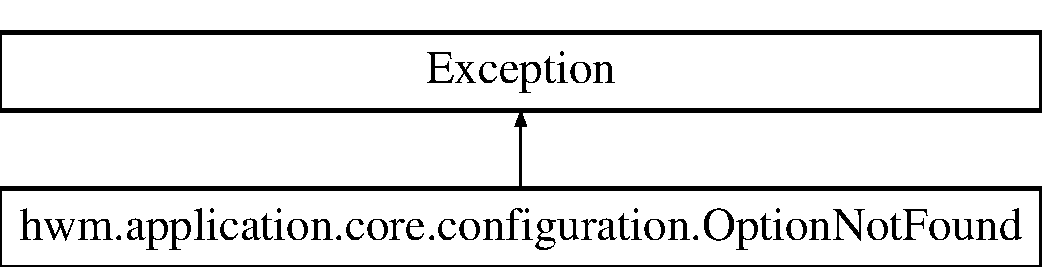
\includegraphics[height=2.000000cm]{classhwm_1_1application_1_1core_1_1configuration_1_1_option_not_found}
\end{center}
\end{figure}


The documentation for this class was generated from the following file\-:\begin{DoxyCompactItemize}
\item 
C\-:/\-Users/\-Jimmy/\-Documents/\-Files/\-Work/\-Active Projects/\-M\-X\-L/mercury2/\-Hardware\-\_\-\-Manager/hwm/application/core/configuration.\-py\end{DoxyCompactItemize}

\hypertarget{classhwm_1_1application_1_1core_1_1configuration_1_1_option_protected}{\section{hwm.\-application.\-core.\-configuration.\-Option\-Protected Class Reference}
\label{classhwm_1_1application_1_1core_1_1configuration_1_1_option_protected}\index{hwm.\-application.\-core.\-configuration.\-Option\-Protected@{hwm.\-application.\-core.\-configuration.\-Option\-Protected}}
}
Inheritance diagram for hwm.\-application.\-core.\-configuration.\-Option\-Protected\-:\begin{figure}[H]
\begin{center}
\leavevmode
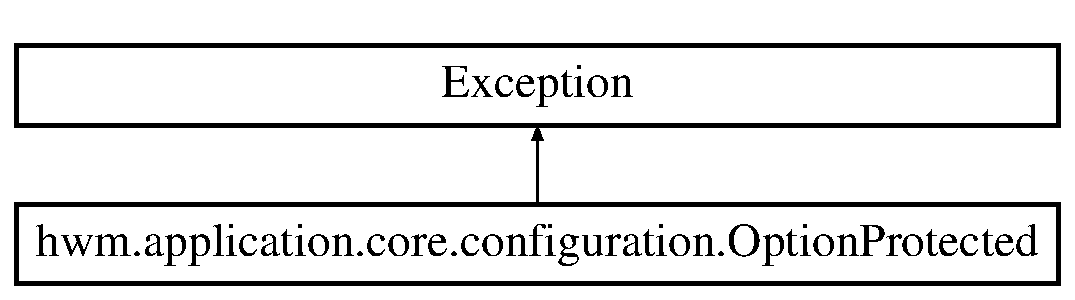
\includegraphics[height=2.000000cm]{classhwm_1_1application_1_1core_1_1configuration_1_1_option_protected}
\end{center}
\end{figure}


The documentation for this class was generated from the following file\-:\begin{DoxyCompactItemize}
\item 
C\-:/\-Users/\-Jimmy/\-Documents/\-Files/\-Work/\-Active Projects/\-M\-X\-L/mercury2/\-Hardware\-\_\-\-Manager/hwm/application/core/configuration.\-py\end{DoxyCompactItemize}

\addcontentsline{toc}{part}{Index}
\printindex
\end{document}
